
\section{Trénovacie dáta}
\label{sec:trenovaciedata}

\subsection{Zber dát}
Pre trénovanie modelov boli použité obrázky zo zdrojov spomenutých v kapitole \ref{sec:databaza}.
Tabuľka nižšie uvádza podrobné počty obrázkov z daných zdrojov ktoré boli použité pre určenie typu zbrane v 2 kategóriách.

\begin{table}[H]
  \centering
  \label{my-label}
  \begin{tabular}{|l|c|c|}
    \hline
    Zdroj               & \multicolumn{1}{l|}{Počet krátkych zbraní} & \multicolumn{1}{l|}{Počet dlhých zbraní} \\ \hline
    IMFDB               & 647                                        & 670                                      \\ \hline
    ImageNet            & 730                                        & 94                                       \\ \hline
    Google vyhľadávanie & 0                                          & 86                                       \\ \hline \hline
    SPOLU               & 1377                                       & 850                                      \\ \hline
  \end{tabular}
  \caption{Podrobné počty trénovacích dát.}
\end{table}

Vo všeobecnosti je jednoduchšie nájsť obrázky ktoré obsahujú krátke zbrane (pištole) ako dlhé zbrane.
Databáza ImageNet obsahovala vyše 3000 odkazov na obrázky, avšak veľká časť z nich bola chybná alebo daný súbor už neexistoval.

Ako bolo spomínane v \ref{subsec:generovanie3d}, obrázky ktoré boli použité na trénovanie modelov pre určenie náklonu zbrane bolo potrebné
    vygenerovať pomocou 3D modelov.
Pre toto generovanie bolo použitých 10 pozadí scény a 5 3D modelov z toho 3 modely boli dlhé zbrane a 2 modely krátkych zbraní.

\begin{figure}[H]
    \centering
    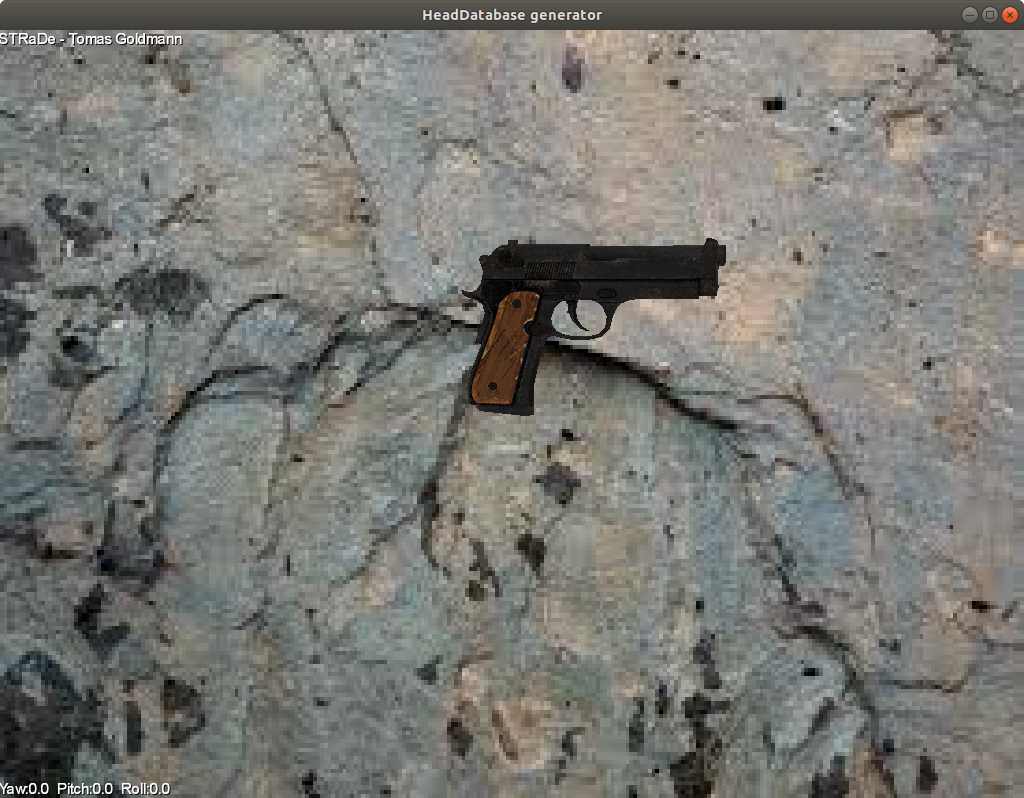
\includegraphics[width=0.7\textwidth]{generator3d}
    \caption{Program pre generovanie obrázkov z 3D modelov.}
    \label{pic:generator3d}
\end{figure}

Niektoré použité modely mali nastavený zlý bod otáčania a taktiež boli veľmi malé.
Preto, ako je vidieť na obrázku \ref{pic:generator3d}, museli byť výsledne obrázky ešte orezané aby sa vnich nachádzala iba zbran bez nepotrebného okolia.

\begin{figure}[H]
    \centering
    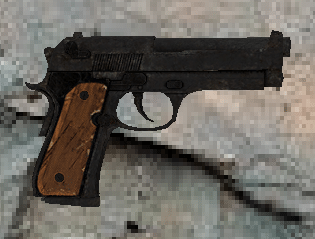
\includegraphics[width=0.5\textwidth]{croped_weapon}
    \caption{Výsledný vygenerovaný obrázok po orezaní okolia.}
    \label{pic:generator3d}
\end{figure}

Tabuľka nižsie uvádza presné počty vygenerovaných obrázkov.

\begin{table}[H]
    \centering
    \label{my-label}
    \begin{tabular}{|l|c|}
        \hline
        Typ osi otáčania & \multicolumn{1}{l|}{Počet obrázkov} \\ \hline
        pitch            & 1480                                \\ \hline
        roll             & 4450                                \\ \hline
        yaw              & 4600                                \\ \hline
        \end{tabular}
    \caption{Podrobné počty trénovacích dát.}
\end{table}

Pre os otáčania pitch boli vybrané obrázky z datasetu určeného pre klasifikáciu typu zbrane.
Pre zvyšné 2 osi boli obrázky generované, počty sa líša kvôli niektorým chybným obrázkom ktoré museli byť vymazané.

\subsection{Načitavanie dát}
\label{subsec:nacitaniedat}
- loader.py - DataLoader a DataSaver
- triedy ktore implementuju nacitavanie dat
- ako sa upravuju data pri nacitani
- Pre nacitanie dat je implemntovane trieda... v scripte ... ktora nacita vstupne obrazky z viacerych moznosti, zo suboru,
  z priecinka kde pre klasifikaciu su urcene labely podla nazvu subfoldra a pre urcenie uhla sa urcuju z nazvu obrazka (diagram ako vyzera struktura foldrov)
  Nasledne je mozne este nacitat len jedne obrazok.

\subsection{Predspracovanie dát}
\label{subsec:predspracovaniedat}
- preprocessing.py - Preprocessor, Preprocessing
- ktore triedy implementujú augmentáciu
- opisat celkovu triedu od Keras-u + Moja vlastne 2 triedy ktore som implementoval
- ako prebiehala augmentacia dat, opisat funkcie ktore sa pouzivaju pre dogenerovanie obrazkov a nazov tried ktore to implementuju.
